\documentclass{article}
\usepackage[a4paper,margin=1in,footskip=0.25in]{geometry}
\usepackage{tikz}
\usetikzlibrary{spy,shapes,shadows,calc,pgfplots.groupplots}
\usepackage{amsmath}
\usepackage{amsfonts}
\usepackage{amssymb}
\usepackage{stmaryrd}
\usepackage{graphicx}
\usepackage{epstopdf}
\usepackage{algorithmic}
\usepackage{enumitem}
\usepackage{booktabs}
\usepackage{pgfplotstable}
\usepackage{colortbl}

\pgfplotstableset{% global config
    every head row/.style={before row=\bottomrule,after row=\hline},
    every last row/.style={after row=\toprule},
}

\providecommand{\abs}[1]{\left\lvert#1\right\rvert}
\providecommand{\norm}[1]{\left\lVert#1\right\rVert}

\newcommand{\drawSquare}{\begin{tikzpicture}
\node[ ] at (0,0) {\textcolor{blue}{\nullfont\pgfuseplotmark{square}}};
\end{tikzpicture} }
\newcommand{\drawCircle}{
\begin{tikzpicture}
\node[ ] at (0,0) {\textcolor{red}{\nullfont\pgfuseplotmark{o}}};
\end{tikzpicture} }
\newcommand{\drawTriangle}{\begin{tikzpicture}
\node[ ] at (0,0) {\textcolor{green!70!black}{\nullfont\pgfuseplotmark{triangle}}};
\end{tikzpicture}
}
\begin{document}


\begin{figure}[h]
\begin{center}
\begin{tikzpicture}[scale = 1.0]
\begin{scope}[ ]
\begin{tiny}
\begin{axis}[
    height = 4.75cm,
    width = 5.7cm,
    name=displ,
    ymode=log,
    xmode=log,
    ymax = 7e-1,
    axis y line*=left,
    xlabel= { $\Delta t = h$},
    x label style={at={(axis description cs:0.55,+0.21)},anchor=east},
    legend style = { column sep = 10pt, legend columns = 1, legend to name = grouplegendn,},
    title = {  $\norm{ u - \mathcal{L}_{\Delta t} \underline{u}_1 }_{L^{\infty}(0,T;L^2(\Omega))}$ }, 
    title style={at={(0.5,1.0735)},anchor=north},
     legend style={at={(0.5,-0.1)},anchor=north},
	]
    
    \addplot[blue,only marks,mark=square,mark options={scale=1.25},forget plot] 
   	table[x=deltat,y=MTM-lo] {../data/precond-3d-noGCC-LinftyL2u-order1.dat}; %\addlegendentry{$q=1$}%   
    \addplot[blue,very thick] 
   	table[x=deltat,y=MTM-lo] {../data/precond-3d-noGCC-LinftyL2u-order1.dat}; \addlegendentry{$q=1$}%   
    \addplot[red,very thick,forget plot] 
   	table[x=deltat,y=DFB] {../data/precond-3d-noGCC-LinftyL2u-order1.dat};    
     \addplot[red,very thick,only marks, mark=o,mark options={scale=1.25},forget plot] 
   	table[x=deltat,y=DFB] {../data/precond-3d-noGCC-LinftyL2u-order1.dat}; 
    
    \addplot[blue,only marks,mark=square,mark options={scale=1.25},forget plot] 
   	table[x=deltat,y=MTM-lo] {../data/precond-3d-noGCC-LinftyL2u-order2.dat}; %\addlegendentry{$q=2$}%    
    \addplot[blue,very thick,dashed] 
   	table[x=deltat,y=MTM-lo] {../data/precond-3d-noGCC-LinftyL2u-order2.dat}; \addlegendentry{$q=2$}%   
     \addplot[red,very thick,only marks, mark=o,mark options={scale=1.25},forget plot] 
   	table[x=deltat,y=DFB] {../data/precond-3d-noGCC-LinftyL2u-order2.dat}; 
    \addplot[red,very thick,dashed,forget plot] 
   	table[x=deltat,y=DFB] {../data/precond-3d-noGCC-LinftyL2u-order2.dat};   

    \addplot[blue,only marks,mark=square,mark options={scale=1.25},forget plot] 
   	table[x=deltat,y=MTM-lo] {../data/precond-3d-noGCC-LinftyL2u-order3.dat}; %\addlegendentry{$q=3$}%   
    \addplot[blue,very thick,densely dotted] 
   	table[x=deltat,y=MTM-lo] {../data/precond-3d-noGCC-LinftyL2u-order3.dat}; \addlegendentry{$q=3$}%   
    \addplot[red,very thick,only marks, mark=o,mark options={scale=1.25},forget plot] 
   	table[x=deltat,y=DFB] {../data/precond-3d-noGCC-LinftyL2u-order3.dat}; 
    \addplot[red,very thick,densely dotted] 
	table[x=deltat,y=DFB] {../data/precond-3d-noGCC-LinftyL2u-order3.dat}; 

    \addplot[lightgray,dashed,ultra thick] 
    	table[mark=none,x=deltat,y expr ={.9*\thisrowno{0}}] {../data/precond-3d-noGCC-LinftyL2u-order1.dat};  %\addlegendentry{$ \mathcal{O}(\Delta t) $ } %
    \addplot[lightgray,dotted,ultra thick] 
    	table[mark=none,x=deltat,y expr ={.35*\thisrowno{0}*\thisrowno{0} }] {../data/precond-3d-noGCC-LinftyL2u-order2.dat};  %\addlegendentry{$ \mathcal{O}((\Delta t)^2) $ } %
    \addplot[lightgray,dashdotted,ultra thick] 
    	table[mark=none,x=deltat,y expr ={.25*\thisrowno{0}*\thisrowno{0}*\thisrowno{0}}] {../data/precond-3d-noGCC-LinftyL2u-order3.dat};  %\addlegendentry{$ \mathcal{O}((\Delta t)^3) $ } %
    %\legend{ $q=k=1$, $q=k=2$,$q=k=3$ } 
    %\node[draw,circle,ultra thick,lightgray] (Z1) at (axis cs:0.0625,6.5e-3) {};
   \end{axis}
    \node at ($(displ) + (-0.0cm,-2.55cm)$) {\ref{grouplegendn}}; 
\end{tiny}
\end{scope}

 \begin{scope}[xshift=4.5cm]
 %\begin{footnotesize}
 \node (geom) at (1.15,2.25) {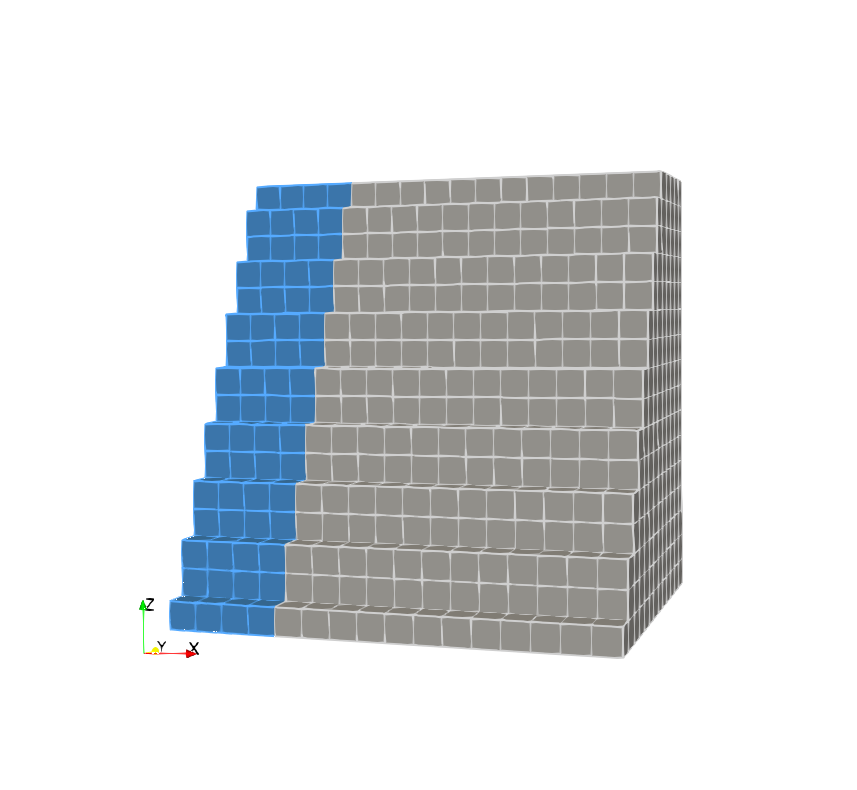
\includegraphics[scale =.13]{noGCC-data-domain-reflvl3.png}};
 \node[draw,fill=white] (la) at (0.46,3.15) { {\footnotesize $\omega $ }};
  \node[] (Z2) at (-2.25,0.55) {};
  \node (err) at (1.0,-0.4) {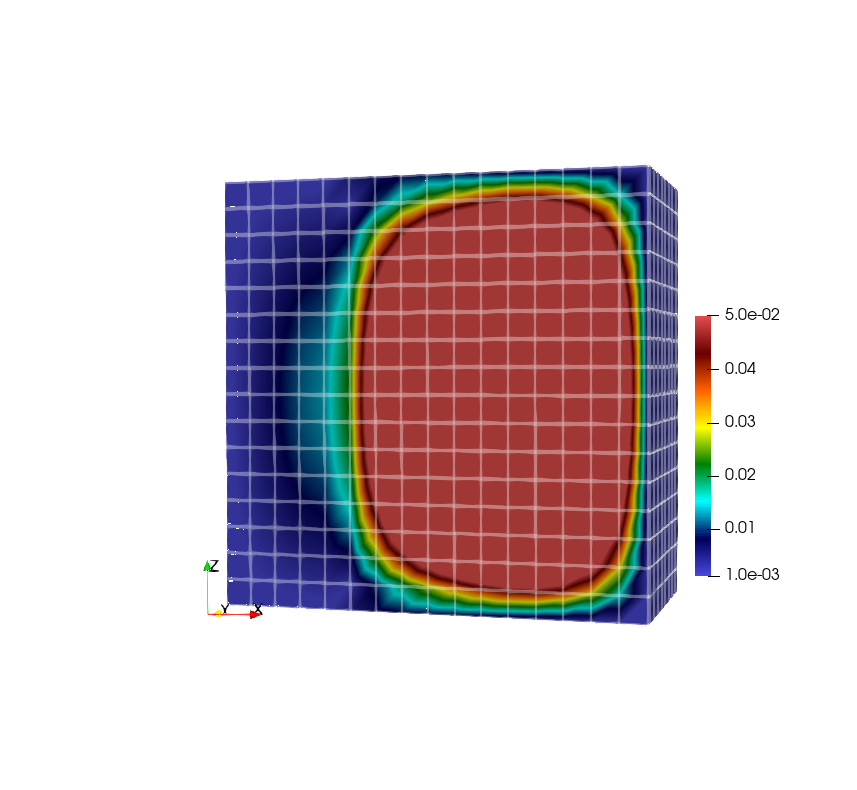
\includegraphics[scale =.13]{noGCC-abserr-displacement-reflvl3.png}};
 \node[draw,fill=white] (la) at (1.05,0.78) {\tiny{$\vert u(0,\cdot) - \mathcal{L}_{\Delta t} \underline{u}_1(0,\cdot) \vert$}};
 \draw[lightgray,ultra thick, ->] (-0.3,-0.55 ) -- (-3.145, 2.195);
 %\end{footnotesize}
 \end{scope}

\begin{scope}[xshift=7.5cm]
\begin{tiny}
\begin{axis}[ 
    height = 4.75cm,
    width = 5.7cm,
    name=vel,
    ymode=log,
    xmode=log,
    ymax = 1e-0,
    xlabel= { $\Delta t = h$},
    axis y line*=left,
    legend style = { column sep = 10pt, legend columns = 1, legend to name = grouplegendnv,},
    x label style={at={(axis description cs:0.55,+0.21)},anchor=east},
    title = {  $\norm{ \partial_t( u - \mathcal{L}_{\Delta t} \underline{u}_1 ) }_{L^{2}(0,T;L^2(\Omega))}$ },
    legend style={at={(0.5,-0.1)},anchor=north}, 
    title style={at={(0.5,1.0735)},anchor=north},
	]
    
    \addplot[lightgray,dashed,ultra thick] 
    	table[mark=none,x=deltat,y expr ={1.3*\thisrowno{0}}] {../data/precond-3d-noGCC-L2L2ut-order1.dat};  \addlegendentry{$ \mathcal{O}(\Delta t) $ } %
    \addplot[lightgray,dotted,ultra thick] 
    	table[mark=none,x=deltat,y expr ={1.4*\thisrowno{0}*\thisrowno{0} }] {../data/precond-3d-noGCC-L2L2ut-order2.dat};  \addlegendentry{$ \mathcal{O}((\Delta t)^2) $ } %
    \addplot[lightgray,dashdotted,ultra thick] 
    	table[mark=none,x=deltat,y expr ={.5*\thisrowno{0}*\thisrowno{0}*\thisrowno{0}}] {../data/precond-3d-noGCC-L2L2ut-order3.dat};  \addlegendentry{$ \mathcal{O}((\Delta t)^3) $ } %
    
    \addplot[blue,only marks,mark=square,mark options={scale=1.25},forget plot] 
   	table[x=deltat,y=MTM-lo] {../data/precond-3d-noGCC-L2L2ut-order1.dat}; %\addlegendentry{$q=1$}%   
    \addplot[blue,very thick,forget plot] 
   	table[x=deltat,y=MTM-lo] {../data/precond-3d-noGCC-L2L2ut-order1.dat}; \addlegendentry{$q=1$}%   
    \addplot[red,very thick,forget plot] 
   	table[x=deltat,y=DFB,forget plot] {../data/precond-3d-noGCC-L2L2ut-order1.dat};    
     \addplot[red,very thick,only marks, mark=o,mark options={scale=1.25},forget plot] 
   	table[x=deltat,y=DFB] {../data/precond-3d-noGCC-L2L2ut-order1.dat}; 
    
    \addplot[blue,only marks,mark=square,mark options={scale=1.25},forget plot] 
   	table[x=deltat,y=MTM-lo] {../data/precond-3d-noGCC-L2L2ut-order2.dat}; %\addlegendentry{$q=2$}%    
    \addplot[blue,very thick,dashed,forget plot] 
   	table[x=deltat,y=MTM-lo] {../data/precond-3d-noGCC-L2L2ut-order2.dat}; \addlegendentry{$q=2$}%   
     \addplot[red,very thick,only marks, mark=o,mark options={scale=1.25},forget plot] 
   	table[x=deltat,y=DFB] {../data/precond-3d-noGCC-L2L2ut-order2.dat}; 
    \addplot[red,very thick,dashed,forget plot] 
   	table[x=deltat,y=DFB] {../data/precond-3d-noGCC-L2L2ut-order2.dat};   

    \addplot[blue,only marks,mark=square,mark options={scale=1.25},forget plot] 
   	table[x=deltat,y=MTM-lo] {../data/precond-3d-noGCC-L2L2ut-order3.dat}; %\addlegendentry{$q=3$}%   
    \addplot[blue,very thick,densely dotted,forget plot] 
   	table[x=deltat,y=MTM-lo] {../data/precond-3d-noGCC-L2L2ut-order3.dat}; \addlegendentry{$q=3$}%   
    \addplot[red,very thick,only marks, mark=o,mark options={scale=1.25},forget plot] 
   	table[x=deltat,y=DFB] {../data/precond-3d-noGCC-L2L2ut-order3.dat}; 
    \addplot[red,very thick,densely dotted,forget plot] 
	table[x=deltat,y=DFB] {../data/precond-3d-noGCC-L2L2ut-order3.dat}; 
 
    %\legend{ $q=k=1$, $q=k=2$,$q=k=3$ } 
    %\node[draw,circle,ultra thick,lightgray] (Z1) at (axis cs:0.0625,6.5e-3) {};
   \end{axis}
    \node at ($(vel) + (-0.0cm,-2.55cm)$) {\ref{grouplegendnv}}; 
\end{tiny}
\end{scope}
\end{tikzpicture}
\end{center}
\vspace{-2.0em}
\begin{center}
$q=k=2$ \\
\pgfplotstabletypeset[ 
    every head row/.style={
    before row={
    \bottomrule
    	& \multicolumn{3}{c}{\textcolor{red}{DFB}} & \multicolumn{3}{c}{\textcolor{blue}{M-l}}\\
	},
	after row=\toprule,
    },
    columns={N,ndof-tot-DFB,ndof-inv-DFB,DFB-iter,ndof-tot-MTM-lo,ndof-inv-MTM-lo,MTM-lo-iter},
    columns/N/.style={  column name={$N$}, column type/.add={>{ \columncolor[gray]{.9} }}{}  },
    columns/ndof-tot-DFB/.style={  column name={ndof-tot}    },
    columns/ndof-inv-DFB/.style={  column name={ndof-inv}    },
    columns/DFB-iter/.style={  column name={iter} },
    columns/ndof-tot-MTM-lo/.style={  column name={ndof-tot}    },
    columns/ndof-inv-MTM-lo/.style={  column name={ndof-inv}    },
    columns/MTM-lo-iter/.style={  column name={iter} },
    ] {../data/precond-3d-noGCC-iters-order2.dat}
\end{center}

\label{fig:NoGCC-3D}
\end{figure}
\end{document}

